% \newcommand{\compacttitlespacing}{0} %disable when we need room for authors
\documentclass[sigconf]{acmart}
\settopmatter{printacmref=false}
% defining the \BibTeX command - from Oren Patashnik's original BibTeX documentation.
\def\BibTeX{{\rm B\kern-.05em{\sc i\kern-.025em b}\kern-.08emT\kern-.1667em\lower.7ex\hbox{E}\kern-.125emX}}
    
\usepackage{nicefrac}
\usepackage{siunitx}
\usepackage{array,framed}
\usepackage{booktabs}
\usepackage{
  color,
  float,
  epsfig,
  wrapfig,
  graphics,
  graphicx,
  subcaption
}
% \usepackage[dvipsnames]{xcolor}
\usepackage{textcomp,amssymb}
\usepackage{setspace}
% \usepackage{amsfonts}
\usepackage{latexsym,fancyhdr,url}
\usepackage{enumerate}
\usepackage{algorithm2e}
\usepackage{algpseudocode}
\usepackage{graphics}
\usepackage{xparse} % argument parsing -- \edist
\usepackage{xspace}
\usepackage{multirow}
\usepackage{csvsimple}
\usepackage{balance}
% \usepackage{flushend}
% \usepackage{mathptmx,avant}

%%%% Tikz variables, pgfplot
\usepackage{
  tikz,
  pgfplots,
  pgfplotstable
}
\usepackage{hyperref}

\usetikzlibrary{
  shapes.geometric,
  arrows,
  external,
  pgfplots.groupplots,
  matrix
}

\pgfplotsset{compat=1.9}
% \tikzexternalize[prefix=images/]
% \tikzexternalenable

%\pagenumbering{arabic}
% \pagestyle{plain}

\usepackage{mathtools,}
\DeclarePairedDelimiter\abs{\lvert}{\rvert}
\DeclarePairedDelimiter\norm{\lVert}{\rVert}

% \setmathfont{Latin Modern Math}[version=lm]
\DeclareMathAlphabet{\mathcal}{OMS}{cmsy}{m}{n}
% \DeclareSymbolFont{operators}{T1}{cmr}{m}{n}
% \DeclareSymbolFont{letters}{OML}{cmm}{m}{it}
% \DeclareSymbolFont{symbols}{OMS}{cmsy}{m}{n}
% \DeclareSymbolFont{largesymbols}{OMX}{cmex}{m}{n}

% \usepackage{times}

% \setmathcal{Arial}

% TO deal with the weird flow of boxes
% \brokenpenalty=1000
% \clubpenalty=1000
% \widowpenalty=10
\DeclareGraphicsExtensions{%
    .png,.PNG,%
    .pdf,.PDF,%
    .jpg,.mps,.jpeg,.jbig2,.jb2,.JPG,.JPEG,.JBIG2,.JB2}

\setlength{\belowcaptionskip}{-10pt} 
\setlength{\footskip}{30pt}
\setlength{\abovecaptionskip}{5pt plus 3pt minus 2pt} 
%%%%%%%%%%%%%%%%%%%%%%%%%%%%%%%%%%%%%%%%%%%%%%%%%%%%%%%%%%%%%%%%%%%%%%%%%%%%%%

\begin{document}
%\fontfamily{lmr}\selectfont
% \def\thetitle{A Practical Way to Generate Strong Keys from Noisy Data}
\fancyhead{}
\def\thetitle{CSC 410 Assignment 1: Raw Data to Feature Space}
\title{\thetitle}

\author{Kidest Mamo}
\affiliation{\small{UNC--Greensboro}}

\date{02/21/2021}


\maketitle

\section{Introduction}
  In this assignment, a set of raw images were transformed into a feature space.

\section{Task 1}
I already had the Anaconda Python Environment on my PC, which comes with the Jupyter Notebook. I didn't install Spyder as I prefer to use the Notebook. I installed openCV with the following command: \begin{verbatim}
    conda install cv2
\end{verbatim}
Image of setup is depicted in Figure 1.

\begin{figure}[h]
  \centering
  \includegraphics[width=\linewidth]{screenshots/Env.png}
  \caption{Programming Environment Setup.}
  \label{fig:programmingEnvironment}
\end{figure}

\section{Task 2}
My three chosen types of fruit are cherry, banana, and Lime. I chose these because they are very distinct from each other in shape and color, and will hopefully be easier to train on. These images were chosen from the FIDS30 dataset (1).
\begin{figure}[h]
  \centering
  \includegraphics[width=\linewidth]{screenshots/chosen.png}
  \caption{Image Data-sets used in this project}
  \label{fig:imageDataset}

\end{figure}
\begin{figure}[h]
  \centering
  \includegraphics[width=\linewidth]{screenshots/imageFolders.png}
  \caption{Exact images used in this assignment. Left to right: cherry, banana, lime.}
  \label{fig:imageFolders}

\end{figure}

\section{Task 3}
In this section suitable Python and OpenCV libraries were added to perform this task and the rest of this assignment. The libraries used are numpy, pandas, matplotlib, and openCV.

\begin{figure}[h]
  \centering
  \includegraphics[width=\linewidth]{screenshots/imports.png}
  \caption{Imported Libraries}
  \label{fig:importedLibraries}
\end{figure}

Then, the three chosen color images were read in and their R, G, and B channel images were displayed. An example result is shown in Figure ~\ref{fig:observationsAndFeatures}.
\begin{figure}[h]
  \centering
  \includegraphics[width=\linewidth]{screenshots/readAndDisplayBGR.png}
  \caption{Reading in images and displaying the r,b,g color channels of image0.}
\end{figure}

They were then converted into gray-scale and displayed while printing out their dimensions as shown in Figure ~\ref{fig:grayscale}.
\begin{figure}[h]
  \centering
  \includegraphics[width=\linewidth]{screenshots/grayScale.png}
  \caption{Display of gray-scale images and their dimensions. From left to right: image0, image1, and image2. }
  \label{fig:grayscale}
\end{figure}

\section{Task 4}
In this section, parametric function was written to reduce the size of the gray-scale images to have height of 256 pixels while maintaining the aspect ratio for the width keeping it divisible by 8. The function and the resulting dimensions of the resized images is shown in Figure ~\ref{fig:resize}.
\begin{figure}[h]
  \centering
  \includegraphics[width=\linewidth]{screenshots/imageResize.png}
  \caption{Resize function and resulting dimensions.}
  \label{fig:resize}
\end{figure}

\section{Task 5}
In this section, a function made to divide each image into blocks of 8x8 pixels. The blocks were then transformed to vectors of size 64. A label was assigned to each feature vector with 0, 1, and 2 for the first, second, and third images, respectively. A spreadsheet was then generated by storing a feature vector per row in the spreadsheet for each image as shown in Figure ~\ref{fig:block}.
\begin{figure}[h]
  \centering
  \includegraphics[width=\linewidth]{screenshots/blockFeatureVectors.png}
  \caption{Function block. Block feature Vector generation for each image.}
  \label{fig:block}
\end{figure}
\section{Task 6}
In this section, a function was made to divide each image into overlapping blocks of 8x8 pixels. The blocks were then transformed to vectors of size 64. A label was assigned to each feature vector with 0, 1, and 2 for the first, second, and third images, respectively. A spreadsheet was then generated by storing a feature vector per row in the spreadsheet for each image as shown in Figure ~\ref{fig:slidingBlock}.
\begin{figure}[h]
  \centering
  \includegraphics[width=\linewidth]{screenshots/slidingBlockFeatureVectors.png}
  \caption{Sliding block function. Sliding feature Vector generation for each image.}
  \label{slidingBlock}
\end{figure}
\section{Task 7}
\begin{itemize}
    \item Is the dataset imbalanced, inaccurate or incomplete?
    \begin{itemize}
        \item The data set is imabalanced due to sized differences in the images, resulting in different number of observations in the feature vectors of each image.And if is specially so for the sliding block feature vectors where the number of observations for image1 were roughly double that of image0. The exact number of observations for each is given in Figure ~\ref{fig:observationsAndFeatures} 
            \begin{figure}[h]
            \centering
            \includegraphics[width=\linewidth]{screenshots/numberObservations.png}
            \caption{Number of observations and features of the feature vectors}
            \label{fig:observationsAndFeatures}
            \end{figure}
        \item The dataset is not inaccurate because all vectors corresponding to each image were labeled with the same value, separate from the others. Thus, there's no inaccurately labeled data.
        \item The dataset is not incomplete. There're no missing values as shown Figure ~\ref{fig:missingValues}
            \begin{figure}[h]
            \centering
            \includegraphics[width=\linewidth]{screenshots/missingValues.png}
            \caption{Number of observations and features of the feature vectors}
            \label{fig:missingValues}
            \end{figure}
    \end{itemize}
    \item Is it a trivial data or possibly a big data? 
        \indent This is a big data. Although it's big in size it's not anything that a modern computer can't handle. It has a decent amount of features, but it's not high dimensional. However, it's very complex and the classes aren't easily separable. Classification can't be done with non-ML methods. Thus this can be considered to be a big data. 
      \item Does it have scalability problem? There aren't/won't be scalability problems in the datasets that are and will be generated in this project because we're keeping the number of features constant. However, if a dataset generated by somehow who sampled their data differently, then there will be some issues.
      \item Are they high dimensional? This dataset is not high dimensional. As shown previously in Figure ~\ref{fig:observationsAndFeatures} each dataset has 64 features and the number of observations in each dataset is much greater than 64.
      \item Do you need to standardize? Do you need to normalize? How do they affect the data characteristics? The data does need to be transformed one of two ways since as shown in the Figure ~\ref{fig:2feature2class}, Figure ~\ref{fig:2feature3class}, Figure ~\ref{fig:3feature2class}, Figure ~\ref{fig:3feature3class} the classes aren't easily separable. Transforming the data might bring out some useful patterns.
      \begin{itemize}
          \item Do you need to normalize? Yes, as shown in the distributions of image0 and image1's distributions in Figure ~\ref{fig:distribution}, the data doesn't follow a Gaussian distribution so normalization could be useful.
            \begin{figure}[h]
            \centering
            \includegraphics[width=\linewidth]{screenshots/distribution.png}
            \caption{image0 and image1 distribution plots.}
            \label{fig:distribution}
            \end{figure}
          \item Do you need to standardize? No, standardization wouldn't be of use since the data doesn't follow a Gaussian distribution.
          \item How do they affect the data characteristics? Standardization and normalization affect the observation characteristics by scaling the values of the observations. Size and volume, as well as any feature and class characteristics remain unaffected.
      \end{itemize}
\end{itemize}

\section{Task 8}
In this section, the feature vectors in image0.csv and image1.csv were first merged to create a feature space for these images. Each feature and label columns were align vertically to generate the correct feature space for these image classes. The placement of the feature vectors were then randomized and saved as a spreadsheet, image01.csv. Similarly the feature vectors in image0.csv, image1.csv, and image2.csv were merged to create a feature space for these images. Again, the placement of the feature vectors was randomized and the result was saved as a spreadsheet, image012.csv. This was repeated to create feature spaces from those of the sliding block feature vectors. A total of four feature spaces were constructed.
\begin{figure}[h]
 \centering
    \includegraphics[width=\linewidth]{screenshots/featureSpaces.png}
    \caption{Construction of the four feature spaces.}
\end{figure}

\section{Task 9}
Two features were selected and the two-dimensional feature space was plotted, labeling the observations by color based on class(feature 64).
One plot for 2 classes. Another for 3 classes.
\begin{figure}[h]
 \centering
    \includegraphics[width=\linewidth]{screenshots/2d2ClassPlot.png}
    \caption{2 feature plot for 2 classes 0 and 1.}
    \label{fig:2feature2class}
\end{figure}
\begin{figure}[h]
 \centering
    \includegraphics[width=\linewidth]{screenshots/2d3ClassPlot.png}
    \caption{2 feature plot for 3 classes 0, 1, and 2}
    \label{fig:2feature3class}
\end{figure}
Three features were then selected and the three-dimensional feature space was plotted, labeling the observations by color based on class(feature 64).
One plot for 2 classes. Another for 3 classes.
\begin{figure}[h]
 \centering
    \includegraphics[width=\linewidth]{screenshots/3d2ClassPlot.png}
    \caption{3 feature plot for 2 classes 0 and 1.}
    \label{fig:3feature2class}
\end{figure}
\begin{figure}[h]
 \centering
    \includegraphics[width=\linewidth]{screenshots/3d3ClassPlot.png}
    \caption{3 feature plot for 3 classes 0, 1, and 2}
    \label{fig:3feature3class}
\end{figure}
None of the features as plotted in the above figures seem easily separated by class. There are too many overlaps.

\section{Task 10}
Appropriate changes were made to the Python code such that it can read any number of images from a folder that consists of many similar images, generate a feature spaces, and generate a spreadsheets for the feature spaces. This function is depicted in Figure ~\ref{fig:folderFeatureSpaceFunction}.
An example is shown in Figure ~\ref{fig:folderFeatureSpaceExample}.
\begin{figure}[h]
 \centering
    \includegraphics[width=\linewidth]{screenshots/folderFeatureSpaceFunction.png}
    \caption{Function for creating feature space from a folder of similar images.}
    \label{fig:folderFeatureSpaceFunction}
\end{figure}
\begin{figure}[h]
 \centering
    \includegraphics[width=\linewidth]{screenshots/folderFeatureSpaceExample.png}
    \caption{Example of creating a feature space from a folder of similar images.}
    \label{fig:folderFeatureSpaceExample}
\end{figure}

\section{Task 11}
\begin{itemize}
    \item Describe the effects of block size on the dimensionality of the feature space and the number of vectors.
    As block size increases, the higher the dimension(more features) and the lower the number of vectors that the feature space will have. The opposite is the case as block size decreases.
    \item Describe how these effect may influence the classifier that divides the domain
    First of all, as we increase the the block size, thus decrease the number of vectors, we're decreasing the number of vectors we have for training the classifier, which isn't ideal. Also, the increase in features, especially when it result in a high dimensional dataset will raise scalability issues and possibly render the results of the classifier useless. And thus, the dataset will first need to be processed to reduce its dimension before feeding it to the classifier.
\end{itemize}

\section{Assignment 2 Introduction}
 In this assignment, classifiers were developed under the four categories of datasets and
evaluated by using suitable qualitative measures, namely, precision and accuracy.

\section{Task 1}
Here, the data domain of the datasets was divided into 80:20, where 80\% is assigned to training datasets and 20\% is assigned to testing datasets. 
Then, two features were selected in each category of training and testing datasets, and their histograms were plotted to see if they follow the same distribution. The same two features were used again to generate scatter plots, color coded by class label. 
The resulting plots for image01's training dataset is show in Figure ~\ref{fig:image01_distri} and Figure ~\ref{fig:image01_train_scatt}.
The mean and variance of the selected features are also listed in Figure ~\ref{fig:image01_mean_}. Looking at both the plots and mean and vaariance values, the features in this case do follow very similar distributions.

\begin{figure}[h]
 \centering
    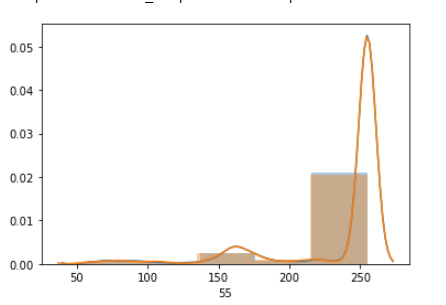
\includegraphics[width=\linewidth]{image01_distribution.png}
    \caption{Distribution plots for the two features of image01_train dataset.}
     \label{fig:image01_distribution}
\end{figure}
\begin{figure}[h]
 \centering
    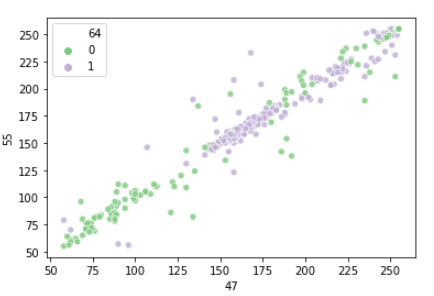
\includegraphics[width=\linewidth]{image01_scatterplot.png}
    \caption{scatter plot of the two features of image01_train dataset.}
     \label{fig:image01_train_scatterplot}
\end{figure}
\begin{figure}[h]
 \centering
    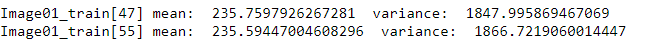
\includegraphics[width=\linewidth]{image01_mean_var.png}
    \caption{mean and variance for the two features of image01_train dataset.}
     \label{fig:image01_mean_var}
\end{figure}

\section{Task 2}
In this task, elastic-net regression was trained and implemented as a two-class classifier using the training sets of the overlapping and non-overlapping feature vectors created in the previous assignment. Only the 2-class datasets were used since this is a 2-class classifier. 
This was achieved using the built in sklearn LogisticRegression model and applying the elastic net penalty on it. The initialization of the models is shown in Figure ~\ref{fig:lasso_initialization}.
After applying the model in the two datasets, a confusion matrix, as shown in Figure ~\ref{fig:lasso_cm} was constructed. From it, the precision and accuracy for each was calculated. The model applied on the overlapping dataset, 'image01s' had a higher accuracy and precision score. Exact values are given in Figure ~\ref{fig:folderFeatureSpaceExample}.

\begin{figure}[h]
 \centering
    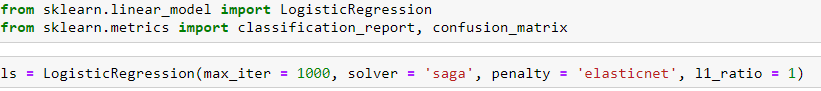
\includegraphics[width=\linewidth]{lasso_initialization.png}
    \caption{Initialization of the lasso classifier.}
     \label{fig:lasso_initialization}
\end{figure}
\begin{figure}[h]
 \centering
    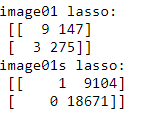
\includegraphics[width=\linewidth]{lasso_cm.png}
    \caption{Confusion matrices from applying the lasso classifier to the 2-class datasets.}
     \label{fig:lasso_cm}
\end{figure}
\begin{figure}[h]
 \centering
    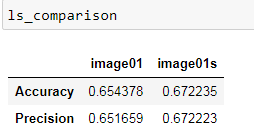
\includegraphics[width=\linewidth]{lasso_performance.png}
    \caption{Precision and accuracy scores for the lasso classifier.}
     \label{fig:lasso_performance}
\end{figure}

\section{Task 3}
In this section, a random forest classifier was trained and implemented as both a 2-class and 3-class classifier using the sklearn.ensemble library. Initialization of the classifier is shown in Figure ~\ref{fig:rfc_initalization}. 
The classifier was trained and applied on all four datasets and a confusion matrix was constructed for each case using the actual and predicted labels. The confusion matrix of each is given in Figure ~\ref{fig:rfc_cm}. 
From there, the precision and accuracy in each was calculated. For the sake of comparison and consistency, the precision on the 3-class datasets was calculated using class 1 as the 'positive' class was the case for the 2-class datasets. The exact values are given in Figure ~\ref{fig:rfc_performance}. Again the classifier performed best on the overlapping 2-class dataset, image01s; it had both the highest accuracy and precision score in this case.

\begin{figure}[h]
 \centering
    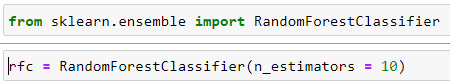
\includegraphics[width=\linewidth]{rfc_intialization.png}
    \caption{Initialization of the random forest classifier.}
     \label{fig:rfc_initalization}
\end{figure}
\begin{figure}[h]
 \centering
    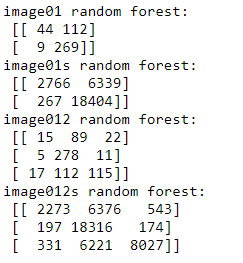
\includegraphics[width=\linewidth]{random_forest_cm.png}
    \caption{Confusion matrices from applying the random forest classifier to the 2-class datasets.}
     \label{fig:rfc_cm}
\end{figure}
\begin{figure}[h]
 \centering
    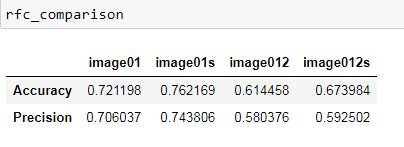
\includegraphics[width=\linewidth]{rfc_performance.png}
    \caption{Precision and accuracy scores for the random forest classifier.}
     \label{fig:rfc_performance}
\end{figure}

\section{Task 4}
The first part of task 4 was examining the difference between the confusion matrix based quantitative measures with the built in measures. The built in measures, accuracy score and precision score were imported from the sklearn.metrics libarary. Figure ~\ref{fig:measures_co} shows how these compare with those calculated from the confusion matrix of the lasso regression models. The biggest difference between the two is in the magnitude of 10e-16, which is insignificant. Thus, it's safe to conclude that there's no significant quantitative difference between the two methods of calculating the accuracy and precision scores.
\begin{figure}[h]
 \centering
    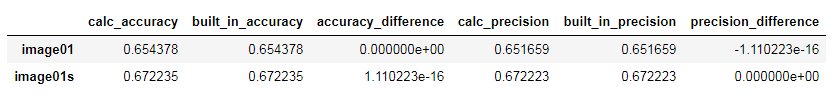
\includegraphics[width=\linewidth]{measures_comp.png}
    \caption{Built-in vs confusion_matrix based measures comparison.}
     \label{fig:measures_comp}
\end{figure}

The second part of task 4 was looking at the performance of all the classifiers across all the datasets to see which pair of classifier and dataset performed best. In part 2, we saw that the lasso regression classifier performed best on the 2-class overlapping dataset, image01s. Same thing in the case of the random forest classifier. Now to determine the better classifier on the image01s dataset, we can see in Figure ~\ref{fig:image01s_comp} that both the accuracy and precision scores are higher for the random forest classifier. Thus, the best classifier-dataset pair is Random Forest Classifier - Image01 Dataset.
\begin{figure}[h]
 \centering
    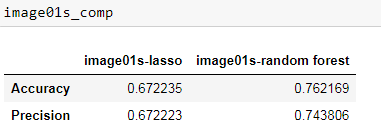
\includegraphics[width=\linewidth]{image01s_comp.png}
    \caption{random forest classifier performance vs lasso classifier performance on image01s dateset.}
     \label{fig:image01s_comp}
\end{figure}

\end{document}


%%% Local Variables:
%%% mode: latex
%%% TeX-master: t
%%% End:
